\documentclass[]{article}
\usepackage{hyperref}
\usepackage{graphicx}
\usepackage{float}
\usepackage{amsmath}
\usepackage{amssymb}
\usepackage[ngerman]{babel}
\usepackage[T1]{fontenc}
\usepackage{lmodern}
\usepackage[utf8]{inputenc} % unter Windows latin1 statt utf8

%opening
\title{Farmrobo}

\author{Jonas Kallweidt und Christian Küllmer}
\date{\today{}, Kassel}

\begin{document}
\maketitle
\begin{figure}[H]
	\centering
	
\includegraphics[width=0.8\textwidth]{DeckblattFarmrobo.jpg}
	\caption{Automatik in der Landwirtschaft}
	\label{img:grafik-dummy}
\end{figure}
\newpage
\tableofcontents


\begin{abstract}
	

\end{abstract}

\section{Vorwort}

	\begin{figure}[H]
	\centering
	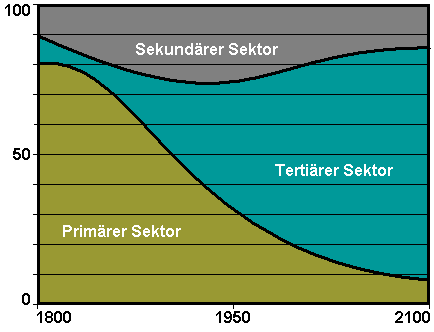
\includegraphics[width=0.8\textwidth]{Fourastie.png}
	\caption{Anzeige der Verteilung von Arbeitskräften zur Zeit \newline
		Quelle: Jean Fourastié: Le Grand Espoir du XXe siècle. Progrès technique, progrès économique, progrès social. Presses Universitaires de France, Paris 1949 = Die große Hoffnung des 20. Jahrhunderts. Köln 1954.}
	\
	\label{img:grafik-dummy}
	
\end{figure} 



Die Konzeption zu automatisiertem Gemüseanbau hat ihren Ursprung in der Tatsache, dass seit der Industrialisierung der Arbeitskräftebedarf der Landwirtschaft zwar schrumpft aber bis heute auf einem stabilen Niveau angekommen ist. Während viele Bereiche des Sekundärsektors durch Maschinen, bei sinkendem Bedarf an Arbeitskraft, bereits größere Produktivität entfalten so ist der Gemüseanbau noch mit großem manuellen Aufwand verbunden. 

Diese Personalkosten haben ein enormes Einsparpotential, während fachlich qualifizierte Spezialisten ihr Fachwissen zu einer breiten Anwendung bringen können.
In dieser Projektarbeit soll gezeigt werden, dass es zu diesem Zeitpunkt noch ein großes Potential bei (ggf. regionalem und von Arbeitskräften unabhängigem) Gemüseanbau gibt, welches durch automatisierten Gemüseanbau nutzbar gemacht werden kann. Es soll untersucht werden, welche Bestandteile für eine Pflanze die wichtigsten Parameter sind um sich entwickeln zu können. Diese Parameter sollen messbar gemacht und die Daten dieser Messung digital gespeichert werden. Diese Speicherbarkeit soll die Einstellung der Parameter möglich machen, wobei sich ebenfalls mit der Wirkbarkeit der Parameter auf die Pflanze beschäftigt werden soll. All dies soll aus dem Hinblick betrachtet werden ein Feld oder einen Zucht Rahmen für Pflanzen vollständig zu automatisieren.

In der aktuellen Forschungsdebatte gibt es bisher keine Möglichkeit automatisiert Gemüse anzubauen. Zwar gibt es Konzepte, wie den Farmbot oder den Farmduino, diese sehen Gemüseanbau allerdings nicht aus der Sicht der vollständigen industriellen Umsetzbarkeit, sondern eher im Hobbybereich einzelne Tätigkeiten Zeit/Software gesteuert an eine Maschine zu übergeben. Diese Konzepte haben allerdings ein großes Potential zu Optimierung. Die Entscheidung eine eigene Maschine zu entwickeln wurde davon bestärkt, dass hier die Möglichkeiten von maschinellem Lernen, Bilderkennung und der vollständigen Automation des Gemüseanbaus Raum gegeben werden kann. Es geht in diesem Projekt darum ein Trägersystem für verschiedenste Implementierungen zu entwickeln. Es soll die Anbindungsmöglichkeit zu neuronalen Netzen der ersten und zweiten Ebene entstehen. Daraus resultieren die Möglichkeiten, dass der Gemüseanbau durch sammlung von Daten stark optimiert und der Output eines Feldes unter umständen stark gesteigert werden kann. Der Ansatz ist von daher neu, weil hier zum ersten mal Formen der E-Technik und der Informatik hier als technisches Mittel Anwendung finden und im Zentrum der Automatisierung stehen. Die Methoden der Agrarkultur-Haltung werden hierbei nur zum Mittel der Pflanzenzucht eingesetzt. 

Motivation:
Warum ist automation in der Landwirtschaft so wichtig?

	\begin{figure}[H]
	\centering
	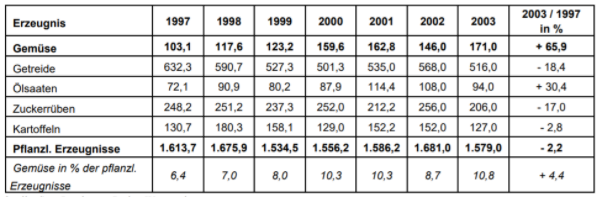
\includegraphics[width=0.8\textwidth]{Tabelle_Daten_Produktion.PNG}
	\caption{Anzeige der Verteilung von Arbeitskräften zur Zeit \newline
		Quelle Statl. Landesamt Baden-Wüttemberg Zitierte Quelle Online im Internet:
		\url{ https://www.lfl.bayern.de/mam/cms07/publikationen/daten/informationen/p_19984.pdf}}
	\label{img:grafik-dummy}
	
\end{figure} 

Es kann festgestellt werden, dass die erlöse der regionalen Landwirtschaft immer weiter steigen. eine weitgehende Automatisierung kann hier zu noch höheren Gewinnspannen führen.

\subsection{Motivation für das Farmrobo Projekt}

\section{Aufbau}

Zur Automatisierung des Gemüsefeldes soll ein Roboter entwickelt werden.

Dieser soll sich sowohl auf einem zweigleisigen Schienensystem an den Rändern des Gemüsefelds, als auch auf einem Querträger bewegen. Diese Anordnung ermöglicht das präzise Zuordnen und Anfahren verschiedener Positionen, indem das Feld als virtuelles Koordinatensystem mit X- und Y-Koordinate unterteilt wird. Dabei lassen sich die unterschiedlichen Richtungen getrennt voneinander messen und regeln. 
Um die Werkzeuge des Roboters an einzelne Pflanzen heran und auch wieder weg zu führen, muss der Roboterarm in der Höhe verstellbar, und somit das Koordinatensystem um eine Z-Koordinate erweitert werden. Der Roboter kann sich nun frei im dreidimensionalen Raum bewegen und dabei die von ihm geforderten Arbeiten (Säen, Gießen, Düngen, Pflegen, Ernten, ...) verrichten. 
Regelung und Arbeitsvorgaben des Roboters sollen mit Hilfe von Software automatisiert ablaufen. Dabei stellt eben genannte Software die Vermittlung zwischen den Anforderungen des Nutzers und dem Roboter dar. Zum einen werden die Wünsche des Nutzers in Form von Steuersignalen an den Roboter geliefert, zum Anderen werden aber auch Messgrößen und Daten gespeichert und dem Nutzer in aufbereiteter Form bereitgestellt. 

Die bei dem nun automatisierten Prozess gesammelten Daten stehen für eine Auswertung, Kalkulation und Prognose sowie Optimierung bereit und sollen in einer Datenbank gesammelt werden, die diese Optimierungen dann im Nachgang ermöglichen soll.

Gesamtaufbau im Überblick:
Aufbau des Schienensystems:
Das Schienensystem legt die Grundlage für die zweidimensionale Abdeckung des Feldes. Dafür sind zwei Metallschienen längs der Ränder vorgesehen, auf denen das Roboterkonstrukt mit Hilfe eines elektrischen Antriebs über das Feld fahren kann. Dieser Aufbau soll das Überfahren und natürlich auch Anhalten an jeder Stelle des Feldes ermöglichen. Dabei ist eine Positionserkennung des Robotergestells vorzusehen.

Es gibt verschiedene Konzepte für den Aufbau der Roboterstruktur und somit auch der Laufschienen. 

Aufbau des Laufwagens: 

Der Laufwagen bedient zunächst zwei Funktionen. Zunächst erweitert er die Bewegungsmöglichkeiten des Krans um eine Bewegung des Wagens quer zur Laufrichtung (wieder unter Zuhilfenahme eines elektrischen Antriebs) der Schienen, sodass nun das Bewegen des Kranwagens in zwei Richtungen möglich ist. 
Darüber hinaus ist der Kranwagen auch für die Höhenregulierung des Werkzeugträgers zuständig. Dafür ist ein Elektromotor vorgesehen, der über ein geeignetes Übersetzungsverhältnis eine Gewindestange antreibt, die dann hoch oder runter fahren kann. 


Aufbau des Werkzeugträgers:
Aufbau der Gießvorrichtung:
Schlauch liefert Wasserzufuhr
Pumpe holt Wasser über Schlauch
Pumpe im Wagen oder Werzeughalter
Tülle zur kontrollierten Bewässerung

Aufbau des Säewerkzeugs:
Idee: Vakuumpumpe
Idee: Schaufelgreifer
Idee. Schnecke

Aufbau des Hakwerkzeugs:
Ideen:
Spitzkeil mit Druck
Häkchen mit Zug
Greifer mit Hub

Aufbau des Düngerwerkzeugs:
ähnlich wie wässern 


Aufbau des Erntewerkzeugs:
Schaufel, Faden, Greifer...

Aufbau der Sensoreinheit:

Die Sensoreinheit soll die wichtigsten Parameter der Pflanzen erfassen. Mit der oben gezeichneten Einheit wird an drei Punkten die Feuchtigkeit des Bodens bestimmt. Des weiteren wird die Temperatur des Bodens und der Luft ermittelt. Diese Werte sind wichtig um die potenziellen Wachstumsprozesse und Bedürfnisse der Pflanzen richtig einzuordnen.
Um die Werte zu erfassen werden kapazitive Sensoren für die Wassererkennung benutzt. Da sich bei einem Wassergefüllten Boden die dielektrischen Werte des Bodens linear zu seinem Dielektrikum ändern, können hier Kapazitive Sensoren benutzt werden. Um die Temperatur zu ermitteln werden konfektionierte Temperatursensoren auf analoge Werte ausgelesen. 

Weiter soll noch die Helligkeit Erfasst werden. Dies soll genutzt werden um die Vorgänge wie z.B. gießen im richtigen Moment durchzuführen. Hierfür wird ein Fototransistor benutzt, der die Helligkeit beinahe Linear anzeigen kann.

Die Berechnung für die Menge der zugeführten Rohstoffe wird dann von diesen Messwerten abhängig diskret ermittelt. Es findet dabei eine Maximierung des Pflanzenwachstums statt, indem aus vergangenen Daten der Datenbank Zukünftige werte Diskret ermittelt und dann abgearbeitet werden. 

Aufbau der Steuerungseinheit:
Die Steuerungseinheit hat besondere anforderungen in der Umgebung einer landwirtschaftlichen Nutzfläche. Hier gilt es vor allem zu beachten, dass die einzelne Aktoren nicht zu einem Ausfall des gesamten Systems führen sollten. Ein Teilausfall soll melde bar sein und die einzelnen Komponenten sollen via drahtloser Kommunikation miteinander sprechen um unnötige Kabelführung am Feldrand zu vermeiden. Die einzelnen Systeme sollen dabei immer in der Wirkung begrenzt sein und nur über die Energieleitungen eine Verbindung zueinander haben. Der Aufbau des Gesamtsystems soll im Funktionsschaubild folgend aussehen:


Aufbau der Stromversorgungseinheit:
5V für Chipsätze/Steuerung
12/24/(230V) Motoren





Zielvorstellung:
Am Ende dieses Projektes soll in Erfahrung gebracht werden, ob es möglich ist, ein System zu bauen, welches automatisiert Gemüse herstellt. Ob das erreicht werden kann, soll die abschließende Projektarbeit klären.


\section{Systemarchitektur}

In diesem Abschnitt wird die Systemarchitektur zur Auswertung und Steuerung des Farmrobos dargestellt.

\subsection{Datenfluss im inneren des Roboters}
Der Farmrobo soll eine selbstlernende Maschine darstellen. Dazu werden Messdaten der Umgebung aufgenommen, aus denen der Farmrobo einen beginnenden Rahmen zu Selbstoptimierung findet. In diesem Kapitel wird dazu der Datenfluss dargestellt, jede Sensorsektion mit den dazugehörigen Messdaten beschildert und dann folgend die Auswertung zum nächsten Steuerungsbefehl angegeben.

	\begin{figure}[H]
	\centering
	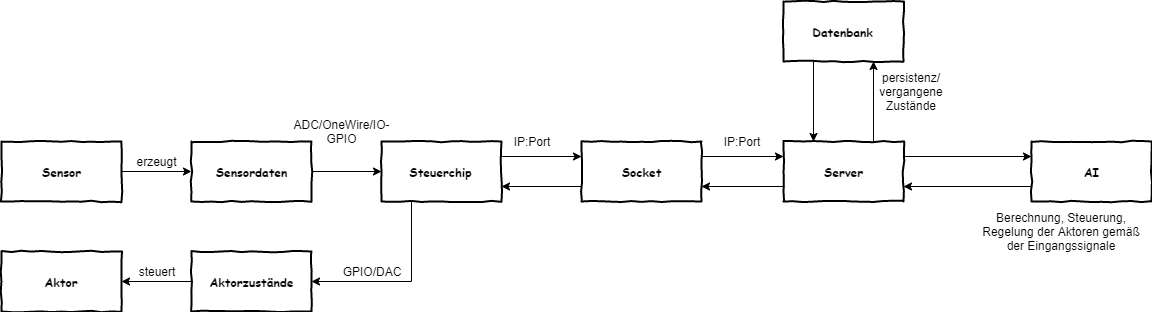
\includegraphics[width=1\textwidth]{Datenflussdiagramm.png}
	\caption{Diese Grafik veranschaulicht den Informations und meldefluss beim Farmrobo}
	\label{img:grafik-dummy}
	\end{figure}
	
Dieser Graph sorgt dafür, dass auf SI-Einheiten oder Zahlenwertgrößen in den Rechenwerken des Farmrobos genutzt werden können.



\subsection{Wassersensor}





\end{document}
